\documentclass[french]{article}
\usepackage[T1]{fontenc}
\usepackage{babel}
\usepackage{hyperref}
\usepackage{graphicx}

\graphicspath{ {./img/} }
\title{%
    \huge Apprendre à gagner au morpion grâce à l'apprentissage par renforcement  \\
    \bigskip
    \large E2 - Cas pratique 1 \\ 
    Développeur en Intelligence Artificielle,
    titre professionnel enregistré au RNCP - École IA Microsoft by Simplon}
\date{19 septembre 2023}
\author{par Vincent Papelard}

\begin{document}
    \maketitle
    \pagenumbering{arabic}
    \pagenumbering{gobble}
    \newpage
    \tableofcontents
    \newpage
    \pagenumbering{arabic}

    \section*{Introduction}
    Ce cas pratique se penche sur l'amélioration d'un modèle d'apprentissage par renforcement appliqué au jeu vidéo. Pour ce faire, nous allons partir d'un modèle que j'ai développé il y a quelques années. Son but ? Apprendre à jouer (et gagner !) à l'un des jeux les plus simples et les plus connus du monde : le morpion.
    
    Dans un premier temps nous ferons un état des lieux du modèle initial et de l'application qui lui est associée. Puis nous parlerons des outils et de la méthodologie utilisés dans le cadre de ce projet avant de présenter les solutions qui ont été mises en oeuvre afin d'améliorer les performances de notre modèle.
    
    Le code associé à ce dossier est disponible sur GitHub : 
    \url{https://github.com/vinpap/tic_tac_toe}.
    \addcontentsline{toc}{section}{Introduction}

    \section{Situation de départ}
    \subsection{L'application}
    Tout d'abord, rappelons les règles du morpion. Deux joueurs s'affrontent sur une grille de 3x3 cases où ils vont, à tour de rôle, choisir une case à occuper (l'un d'entre eux tracera souvent des croix, et l'autre des cercles). L'objectif est de réussir à aligner trois de ses symboles à l'horizontale, à la verticale ou en diagonale, tout en empêchant son adversaire d'en faire autant. La partie s'arrête lorsque l'un des joueurs y parvient, ou si toute la grille est remplie (auquel cas la partie s'achève par un match nul). 

    L'application de départ est bâtie autour de plusieurs composants :
    \begin{itemize}
        \item Une classe qui implémente la logique des règles du jeu et gère l'exécution des parties
        \item Une classe qui affiche une interface réalisée à l'aide du package Python PyGame. Celle-ci permet de visualiser en temps réel le déroulement des parties lorsque deux IA jouent ensemble, ou de jouer soi-même contre une IA
        \item Un ensemble de classes qui héritent d'une interface commune nommée PlayerInterface qui leur permet d'interagir avec le système de jeu. Dans la logique du programme, ces classes représentent des joueurs (humains ou IA) que l'on peut faire jouer en les enregistrant auprès du système de jeu à l'aide d'un simple appel de méthode. Cette structure nous permet d'ajouter facilement de nouveaux modèles d'IA à notre application.
    \end{itemize}

    \begin{figure}[h]
        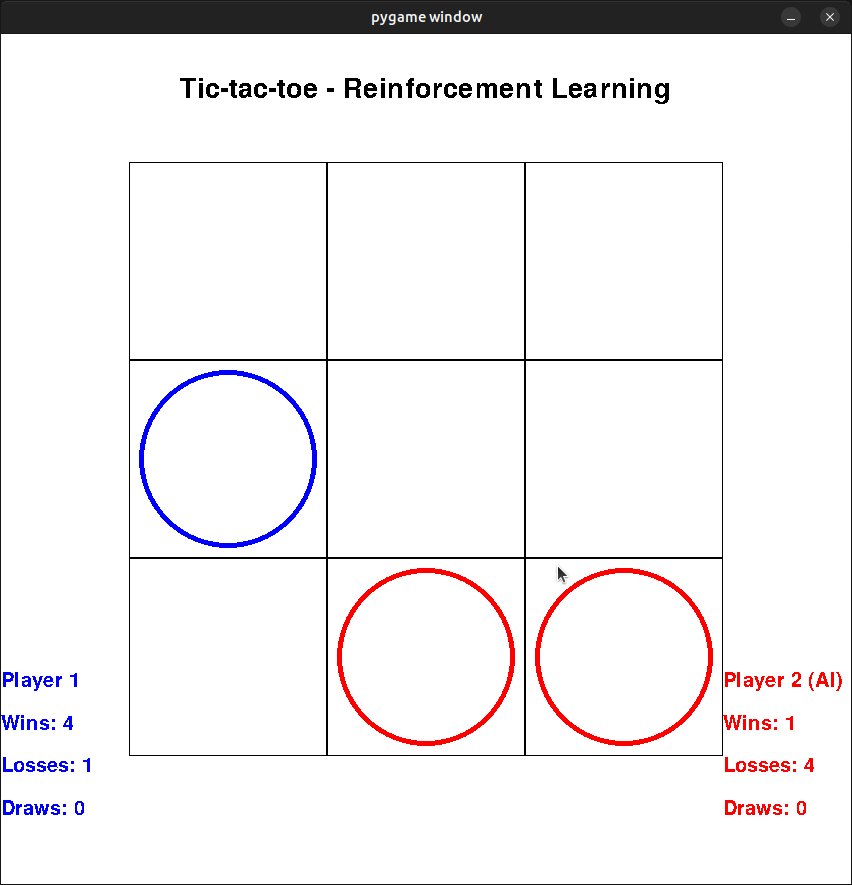
\includegraphics[width=7cm]{game_screenshot}
        \centering
        \caption{Une capture d'écran de l'interface du jeu, ici lors d'une partie entre un joueur humain et une IA}
        \centering
    \end{figure}
    \subsection{Le modèle}
    \subsubsection{Fonctionnement}
    \subsubsection{Performances de départ}

    \section{Outils et méthodologie}
    \subsubsection{Gestion de projet}
    \subsubsection{Outils}
    \subsubsection{Métriques}

    \section{Première tentative d'amélioration : le deep Q-learning}
    \subsubsection{Principe}
    \subsubsection{Implémentation}
    \subsubsection{Résultats}

    \section{Deuxième tentative d'amélioration : modification du modèle de Q-learning pour utiliser un learning rate variable}
    \subsection{Principe}
    \subsection{Implémentation}
    \subsection{Résultats}

    \section{Bilan et leçons à tirer}
    \subsection{Rétrospective sur la gestion de projet}
    \subsection{Les grandes difficultés rencontrées}

    \section{Conclusion}

    \section*{Bibliographie}
    \addcontentsline{toc}{section}{Bibliographie}

\end{document}